% !TEX root = ../presentation.tex
% !BIB program = biber
% !TEX program = xelatex


\begin{frame}
    \frametitle{Types of self-supervised speech representation learning methods}
    
    Schematic of self-supervised methods. Each subfigure illustrates the loss computation for a single time-step. The temporal subscript has been left out for simplicity.

    % \resizebox*{\textheight}{!}{%
        \begin{figure}
            \centering
            \setlength\tabcolsep{1.5pt}
            \begin{tabular}{>{\centering\arraybackslash} m{4mm}  >{\centering\arraybackslash} m{0.40\textwidth}|>{\centering\arraybackslash} m{0.40\textwidth}}
                & {\small \textsc{predictive}} & {\small \textsc{masking-based}} \\
                \rotatebox{90}{{\small \textsc{reconstruct}}} & 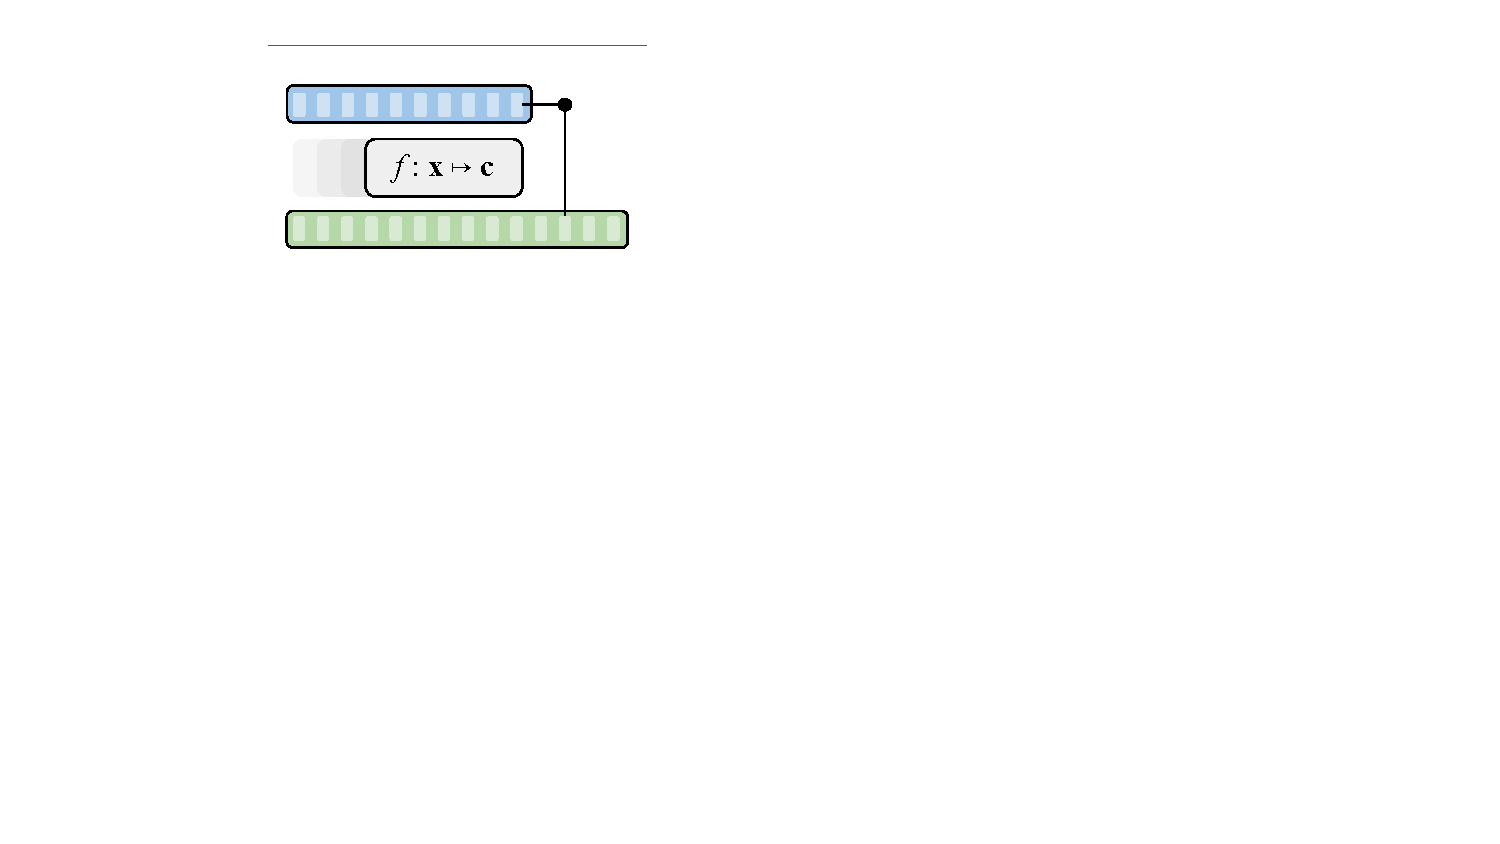
\includegraphics[width=0.40\textwidth]{../graphics/paper_brief/REC_PRD.pdf} & 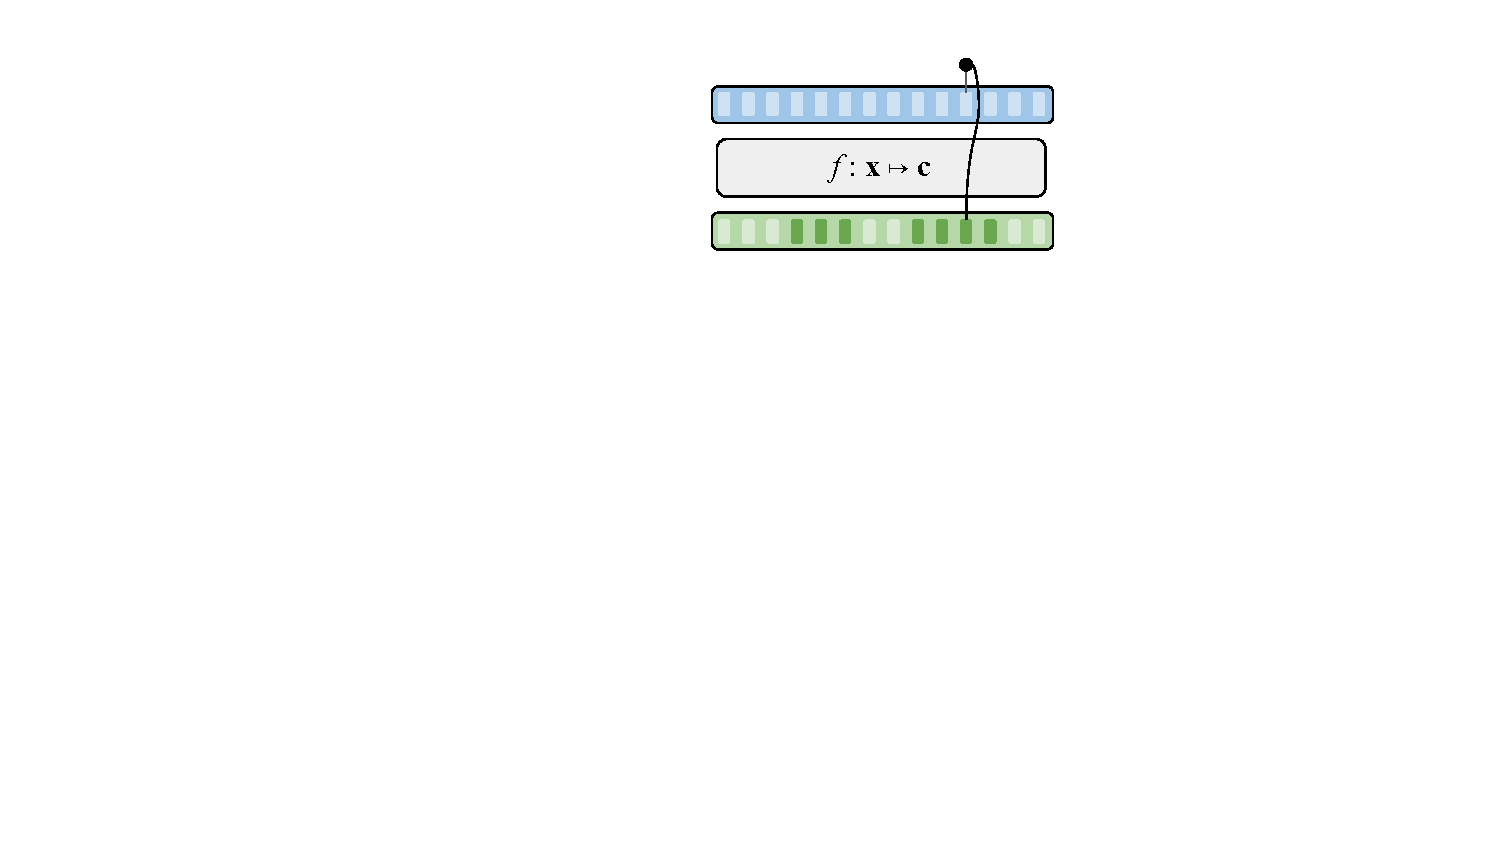
\includegraphics[width=0.40\textwidth]{../graphics/paper_brief/REC_MSK.pdf}  \\
                \midrule
                \rotatebox{90}{{\small \textsc{contrastive}}} & 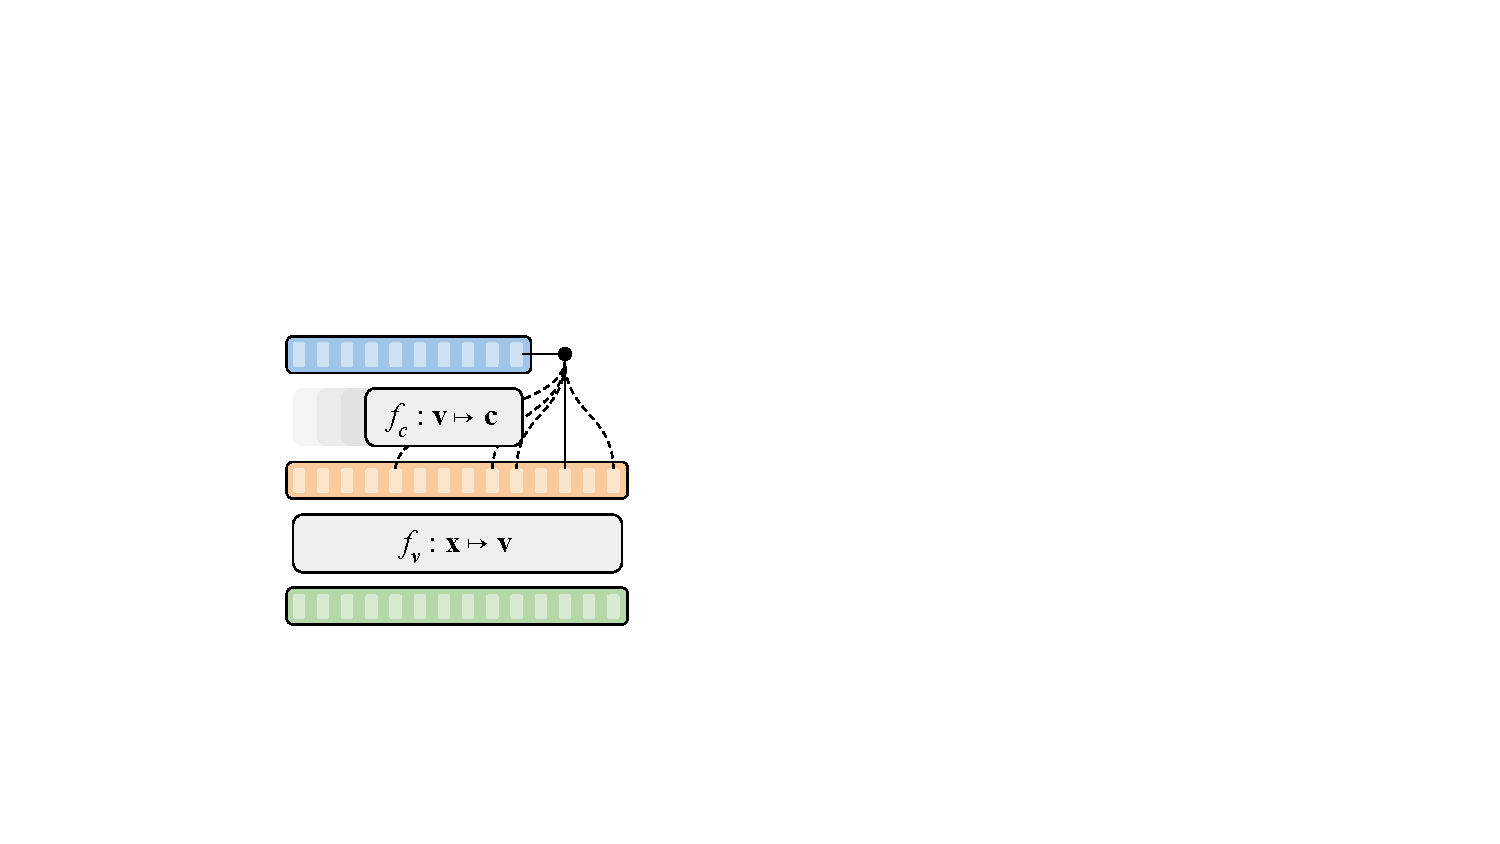
\includegraphics[width=0.40\textwidth]{../graphics/paper_brief/CON_PRD.pdf} & 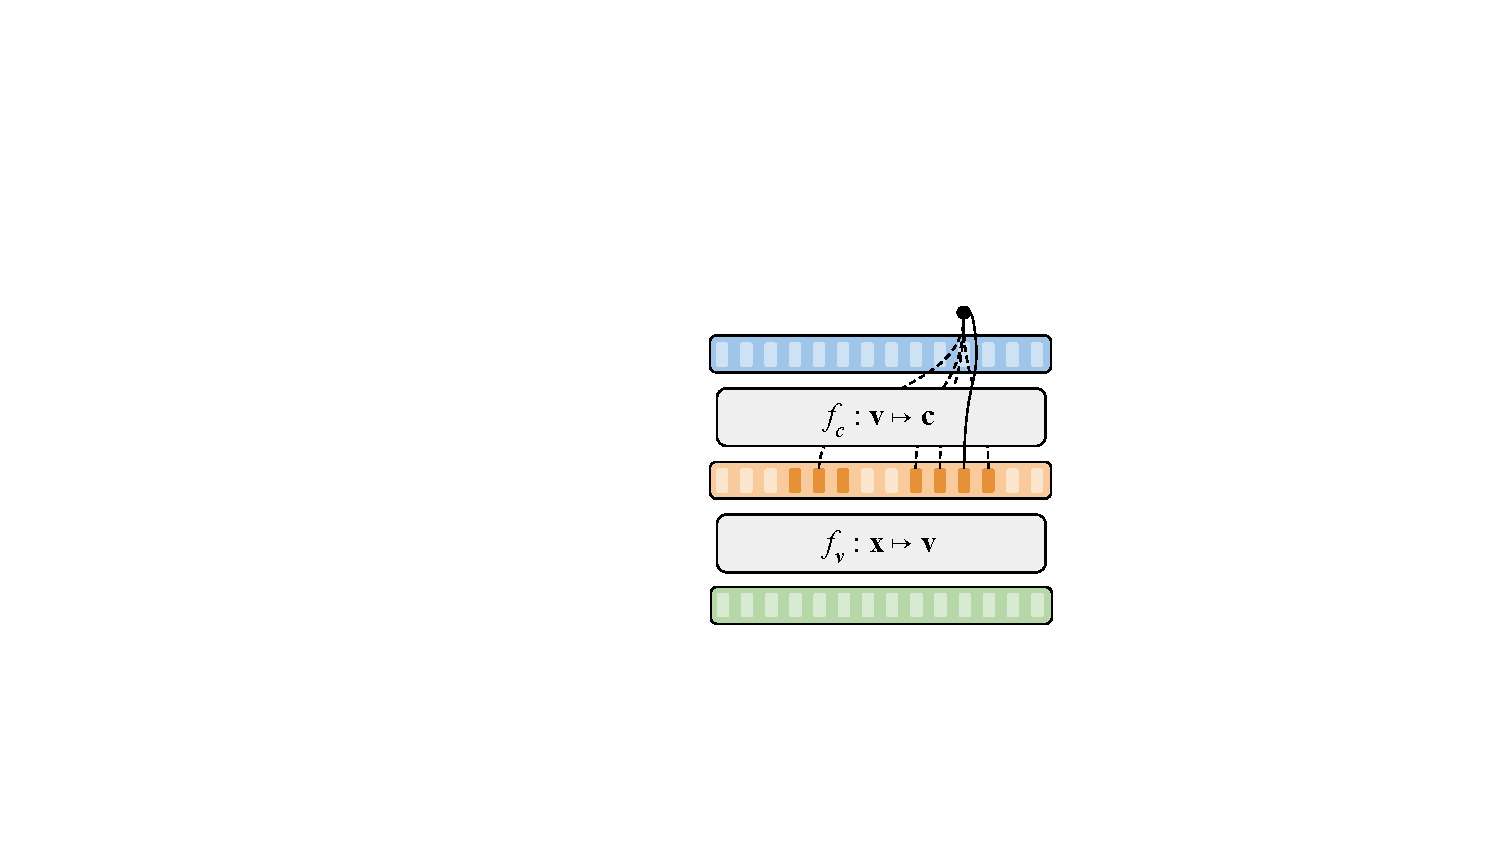
\includegraphics[width=0.40\textwidth]{../graphics/paper_brief/CON_MSK.pdf}
            \end{tabular}
        \end{figure}
    % }
\end{frame}
